I componenti del gruppo dovranno rivestire ciascuno, almeno una volta, tutti i ruoli di progetto indicati nella sezione A.4 . Durante le varie fasi un componente può rivestire anche più ruoli contemporaneamente, purchè non si presentino casi di conflitti come descritto in \textit{Norme di Progetto v1.0.0} .

\noindent Nelle sezioni successive si elencherà nel dettaglio la suddivisione del lavoro dei componenti nelle varie fasi di progetto.

\subsection{Analisi}
Nella macro-fase di \textbf{Analisi} ciascun componente del gruppo dovrà rivestire i ruoli elencati nella seguente tabella:

\begin{table}[h]
\centering
\begin{tabular}{|l|c|c|c|c|c|c|c|}
\toprule
	\textbf{Cognome e Nome} & \multicolumn{6}{c}{\textbf{Ore per ruolo}} & \textbf{Ore Totali} \\
	& \textbf{Re} & \textbf{Am} & \textbf{An} & \textbf{Pt} & \textbf{Pr} & \textbf{Ve} & \\
	 
\midrule
	Agostinetto Matteo & 3 & & 16 & & & 3 & 22 \\
	Burlin Valerio & 14 & & & & & 8 & 22 \\ 
	Carraro Nicola & & & 16 & & & 6 & 22 \\
	Crespan Emanuele & & 14 & & & & 7 & 21 \\
	Ros Fabio & & & 18 & & & 3 & 21 \\
	Suierica Bogdan & & 12 & & & & 10 & 22 \\

\bottomrule
\end{tabular}
\caption{Ore a componente per ruolo, Analisi}
\end{table}

\noindent I valori sono riassunti nel seguente grafico, che rappresenta in maniera visiva per quante ore un membro abbia ricoperto un determinato ruolo:

\begin{figure}[h]
\centering
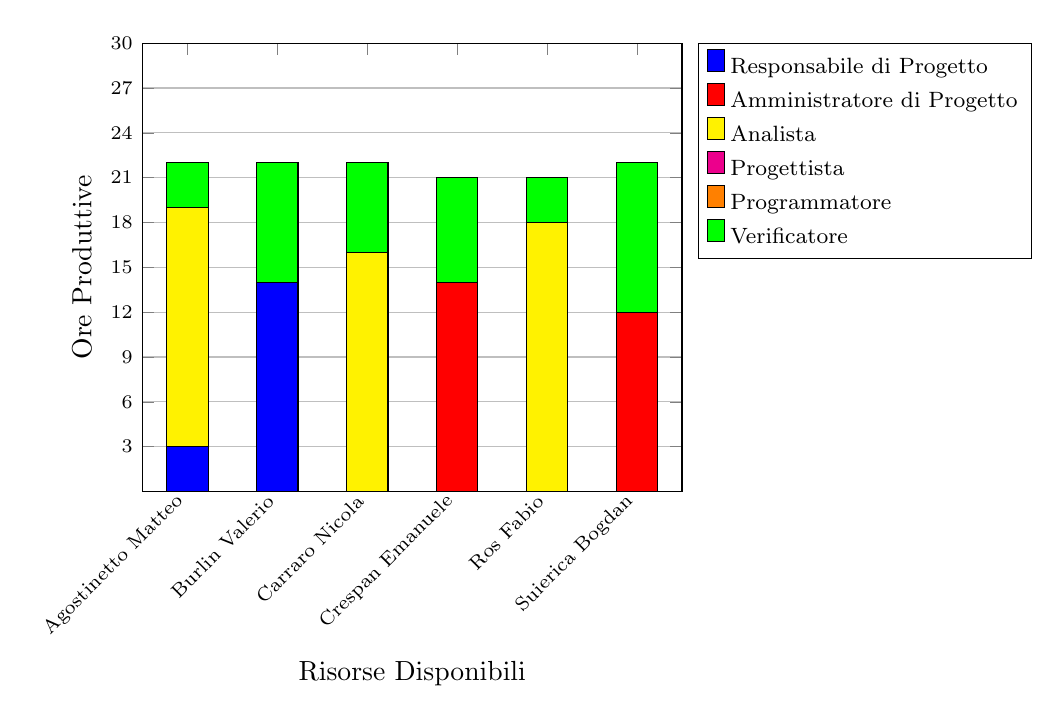
\begin{tikzpicture}
\begin{axis}[
	legend pos = outer north east,
	legend style = {nodes=right,font=\footnotesize},
	ybar stacked,
	bar width = 15pt,
	xlabel = {Risorse Disponibili},
	ylabel = {Ore Produttive},
	tick label style = {font=\scriptsize},
	symbolic x coords = {Agostinetto Matteo,Burlin Valerio,Carraro Nicola,Crespan Emanuele,Ros Fabio,Suierica Bogdan},
	xtick = data,
	x tick label style = {rotate=45,anchor=east},
	ytick = {3,6,9,12,15,18,21,24,27,30},
	ymajorgrids = true,
	ymin = 0,
	ymax = 30]
	\addplot+[ybar,fill = blue,draw = black]
	plot coordinates {(Agostinetto Matteo, 3) (Burlin Valerio, 14) (Carraro Nicola, 0) (Crespan Emanuele, 0) (Ros Fabio, 0) (Suierica Bogdan, 0)};
	\addplot+[ybar,fill = red,draw = black]
	plot coordinates {(Agostinetto Matteo, 0) (Burlin Valerio, 0) (Carraro Nicola, 0) (Crespan Emanuele, 14) (Ros Fabio, 0) (Suierica Bogdan, 12)};
	\addplot+[ybar,fill = yellow,draw = black]
	plot coordinates {(Agostinetto Matteo, 16) (Burlin Valerio, 0) (Carraro Nicola, 16) (Crespan Emanuele, 0) (Ros Fabio, 18) (Suierica Bogdan, 0)};
	\addplot+[ybar,fill = magenta,draw = black]
	plot coordinates {(Agostinetto Matteo, 0) (Burlin Valerio, 0) (Carraro Nicola, 0) (Crespan Emanuele, 0) (Ros Fabio, 0) (Suierica Bogdan, 0)};
	\addplot+[ybar,fill = orange,draw = black]
	plot coordinates {(Agostinetto Matteo, 0) (Burlin Valerio, 0) (Carraro Nicola, 0) (Crespan Emanuele, 0) (Ros Fabio, 0) (Suierica Bogdan, 0)};
	\addplot+[ybar,fill = green,draw = black]
	plot coordinates {(Agostinetto Matteo, 3) (Burlin Valerio, 8) (Carraro Nicola, 6) (Crespan Emanuele, 7) (Ros Fabio, 3) (Suierica Bogdan, 10)};
	\legend{\strut Responsabile di Progetto, \strut Amministratore di Progetto, \strut Analista, \strut Progettista, \strut Programmatore, \strut Verificatore}
\end{axis}
\end{tikzpicture}
\caption{Ore a componente, Analisi}
\end{figure}
\newpage
\subsection{Analisi di Dettaglio}
Nella macro-fase di \textbf{Analisi di Dettaglio} ciascun componente del gruppo dovrà rivestire i ruoli elencati nella seguente tabella:

\begin{table}[h]
	\centering
	\begin{tabular}{|l|c|c|c|c|c|c|c|}
		\toprule
		\textbf{Cognome e Nome} & \multicolumn{6}{c}{\textbf{Ore per ruolo}} & \textbf{Ore Totali} \\
		& \textbf{Re} & \textbf{Am} & \textbf{An} & \textbf{Pt} & \textbf{Pr} & \textbf{Ve} & \\
		
		\midrule
		Agostinetto Matteo & & & & & & 6 & 6 \\
		Burlin Valerio & & & 6 & & & 2 & 8 \\ 
		Carraro Nicola & & 4 & & & & 2 & 6 \\
		Crespan Emanuele & & & 6 & & & & 6 \\
		Ros Fabio & 4 & & & & & 2 & 6 \\
		Suierica Bogdan & & & 6 & & & & 6 \\
		
		\bottomrule
	\end{tabular}
	\caption{Ore a componente per ruolo, Analisi di Dettaglio}
\end{table}

\noindent I valori sono riassunti nel seguente grafico, che rappresenta in maniera visiva per quante ore un membro abbia ricoperto un determinato ruolo:

\begin{figure}[h]
\centering
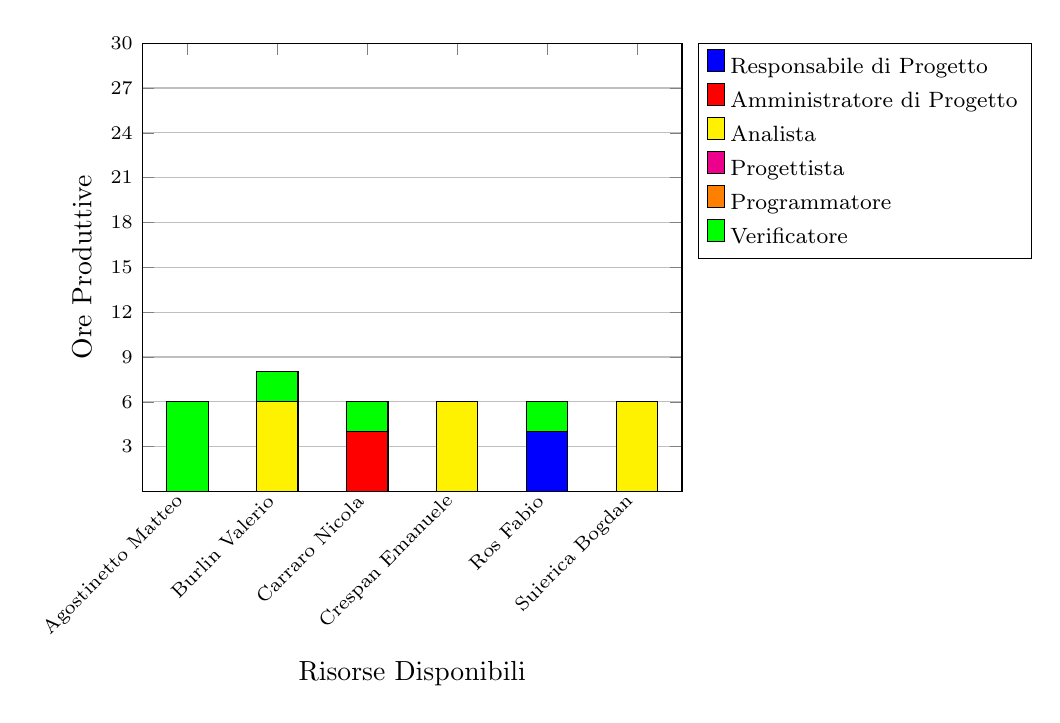
\begin{tikzpicture}
\begin{axis}[
	legend pos = outer north east,
	legend style = {nodes=right,font=\footnotesize},
	ybar stacked,
	bar width = 15pt,
	xlabel = {Risorse Disponibili},
	ylabel = {Ore Produttive},
	tick label style = {font=\scriptsize},
	symbolic x coords = {Agostinetto Matteo,Burlin Valerio,Carraro Nicola,Crespan Emanuele,Ros Fabio,Suierica Bogdan},
	xtick = data,
	x tick label style = {rotate=45,anchor=east},
	ytick = {3,6,9,12,15,18,21,24,27,30},
	ymajorgrids = true,
	ymin = 0,
	ymax = 30]
	\addplot+[ybar,fill = blue,draw = black]
	plot coordinates {(Agostinetto Matteo, 0) (Burlin Valerio, 0) (Carraro Nicola, 0) (Crespan Emanuele, 0) (Ros Fabio, 4) (Suierica Bogdan, 0)};
	\addplot+[ybar,fill = red,draw = black]
	plot coordinates {(Agostinetto Matteo, 0) (Burlin Valerio, 0) (Carraro Nicola, 4) (Crespan Emanuele, 0) (Ros Fabio, 0) (Suierica Bogdan, 0)};
	\addplot+[ybar,fill = yellow,draw = black]
	plot coordinates {(Agostinetto Matteo, 0) (Burlin Valerio, 6) (Carraro Nicola, 0) (Crespan Emanuele, 6) (Ros Fabio, 0) (Suierica Bogdan, 6)};
	\addplot+[ybar,fill = magenta,draw = black]
	plot coordinates {(Agostinetto Matteo, 0) (Burlin Valerio, 0) (Carraro Nicola, 0) (Crespan Emanuele, 0) (Ros Fabio, 0) (Suierica Bogdan, 0)};
	\addplot+[ybar,fill = orange,draw = black]
	plot coordinates {(Agostinetto Matteo, 0) (Burlin Valerio, 0) (Carraro Nicola, 0) (Crespan Emanuele, 0) (Ros Fabio, 0) (Suierica Bogdan, 0)};
	\addplot+[ybar,fill = green,draw = black]
	plot coordinates {(Agostinetto Matteo, 6) (Burlin Valerio, 2) (Carraro Nicola, 2) (Crespan Emanuele, 0) (Ros Fabio, 2) (Suierica Bogdan, 0)};
	\legend{\strut Responsabile di Progetto, \strut Amministratore di Progetto, \strut Analista, \strut Progettista, \strut Programmatore, \strut Verificatore}
\end{axis}
\end{tikzpicture}
\caption{Ore a componente, Analisi di Dettaglio}
\end{figure}
\newpage
\subsection{Progettazione Architetturale}
Nella macro-fase di \textbf{Progettazione Architetturale} ciascun componente del gruppo dovrà rivestire i ruoli elencati nella seguente tabella:

\begin{table}[h]
	\centering
	\begin{tabular}{|l|c|c|c|c|c|c|c|}
		\toprule
		\textbf{Cognome e Nome} & \multicolumn{6}{c}{\textbf{Ore per ruolo}} & \textbf{Ore Totali} \\
		& \textbf{Re} & \textbf{Am} & \textbf{An} & \textbf{Pt} & \textbf{Pr} & \textbf{Ve} & \\
		
		\midrule
		Agostinetto Matteo & & 5 & & 16 & & 7 & 28 \\
		Burlin Valerio & & & 8 & 16 & & 4 & 28 \\ 
		Carraro Nicola & 5 & & & 18 & & 5 & 28 \\
		Crespan Emanuele & & & & 18 & & 9 & 27 \\
		Ros Fabio & & & & 18 & & 9 & 27 \\
		Suierica Bogdan & & & 8 & 14 & & 7 & 29 \\
		
		\bottomrule
	\end{tabular}
	\caption{Ore a componente per ruolo, Progettazione Architetturale}
\end{table}

\noindent I valori sono riassunti nel seguente grafico, che rappresenta in maniera visiva per quante ore un membro abbia ricoperto un determinato ruolo:

\begin{figure}[h]
\centering
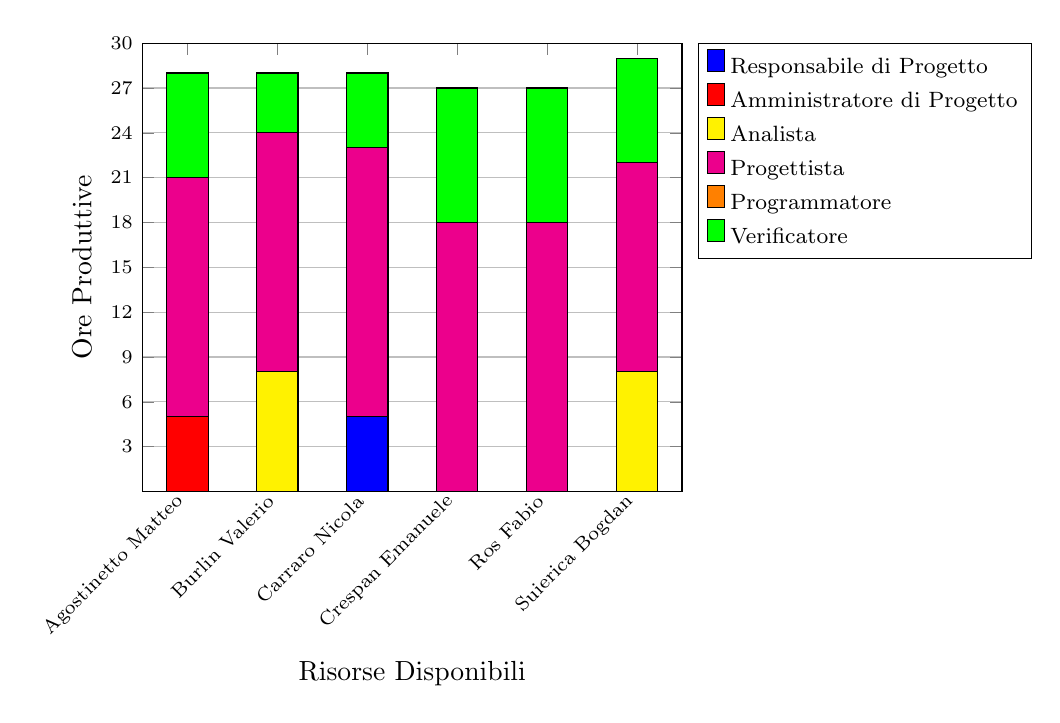
\begin{tikzpicture}
\begin{axis}[
	legend pos = outer north east,
	legend style = {nodes=right,font=\footnotesize},
	ybar stacked,
	bar width = 15pt,
	xlabel = {Risorse Disponibili},
	ylabel = {Ore Produttive},
	tick label style = {font=\scriptsize},
	symbolic x coords = {Agostinetto Matteo,Burlin Valerio,Carraro Nicola,Crespan Emanuele,Ros Fabio,Suierica Bogdan},
	xtick = data,
	x tick label style = {rotate=45,anchor=east},
	ytick = {3,6,9,12,15,18,21,24,27,30},
	ymajorgrids = true,
	ymin = 0,
	ymax = 30]
	\addplot+[ybar,fill = blue,draw = black]
	plot coordinates {(Agostinetto Matteo, 0) (Burlin Valerio, 0) (Carraro Nicola, 5) (Crespan Emanuele, 0) (Ros Fabio, 0) (Suierica Bogdan, 0)};
	\addplot+[ybar,fill = red,draw = black]
	plot coordinates {(Agostinetto Matteo, 5) (Burlin Valerio, 0) (Carraro Nicola, 0) (Crespan Emanuele, 0) (Ros Fabio, 0) (Suierica Bogdan, 0)};
	\addplot+[ybar,fill = yellow,draw = black]
	plot coordinates {(Agostinetto Matteo, 0) (Burlin Valerio, 8) (Carraro Nicola, 0) (Crespan Emanuele, 0) (Ros Fabio, 0) (Suierica Bogdan, 8)};
	\addplot+[ybar,fill = magenta,draw = black]
	plot coordinates {(Agostinetto Matteo, 16) (Burlin Valerio, 16) (Carraro Nicola, 18) (Crespan Emanuele, 18) (Ros Fabio, 18) (Suierica Bogdan, 14)};
	\addplot+[ybar,fill = orange,draw = black]
	plot coordinates {(Agostinetto Matteo, 0) (Burlin Valerio, 0) (Carraro Nicola, 0) (Crespan Emanuele, 0) (Ros Fabio, 0) (Suierica Bogdan, 0)};
	\addplot+[ybar,fill = green,draw = black]
	plot coordinates {(Agostinetto Matteo, 7) (Burlin Valerio, 4) (Carraro Nicola, 5) (Crespan Emanuele, 9) (Ros Fabio, 9) (Suierica Bogdan, 7)};
	\legend{\strut Responsabile di Progetto, \strut Amministratore di Progetto, \strut Analista, \strut Progettista, \strut Programmatore, \strut Verificatore}
\end{axis}
\end{tikzpicture}
\caption{Ore a componente, Progettazione Architetturale}
\end{figure}
\newpage
\subsection{Progettazione di Dettaglio e Codifica}
Nella macro-fase di \textbf{Progettazione di Dettaglio e Codifica} ciascun componente del gruppo dovrà rivestire i ruoli elencati nella seguente tabella:

\begin{table}[h]
	\centering
	\begin{tabular}{|l|c|c|c|c|c|c|c|}
		\toprule
		\textbf{Cognome e Nome} & \multicolumn{6}{c}{\textbf{Ore per ruolo}} & \textbf{Ore Totali} \\
		& \textbf{Re} & \textbf{Am} & \textbf{An} & \textbf{Pt} & \textbf{Pr} & \textbf{Ve} & \\
		
		\midrule
		Agostinetto Matteo & & & & & 38 & 14 & 52 \\
		Burlin Valerio & & 4 & & 12 & 24 & 12 & 52 \\ 
		Carraro Nicola & & & & 4 & 32 & 16 & 52 \\
		Crespan Emanuele & & & 4 & 18 & 24 & 8 & 54 \\
		Ros Fabio & & & & 18 & 24 & 10 & 52 \\
		Suierica Bogdan & 4 & & & 12 & 32 & 6 & 54 \\
		
		\bottomrule
	\end{tabular}
	\caption{Ore a componente per ruolo, Progettazione di Dettaglio e Codifica}
\end{table}

\noindent I valori sono riassunti nel seguente grafico, che rappresenta in maniera visiva per quante ore un membro abbia ricoperto un determinato ruolo:

\begin{figure}[h]
\centering
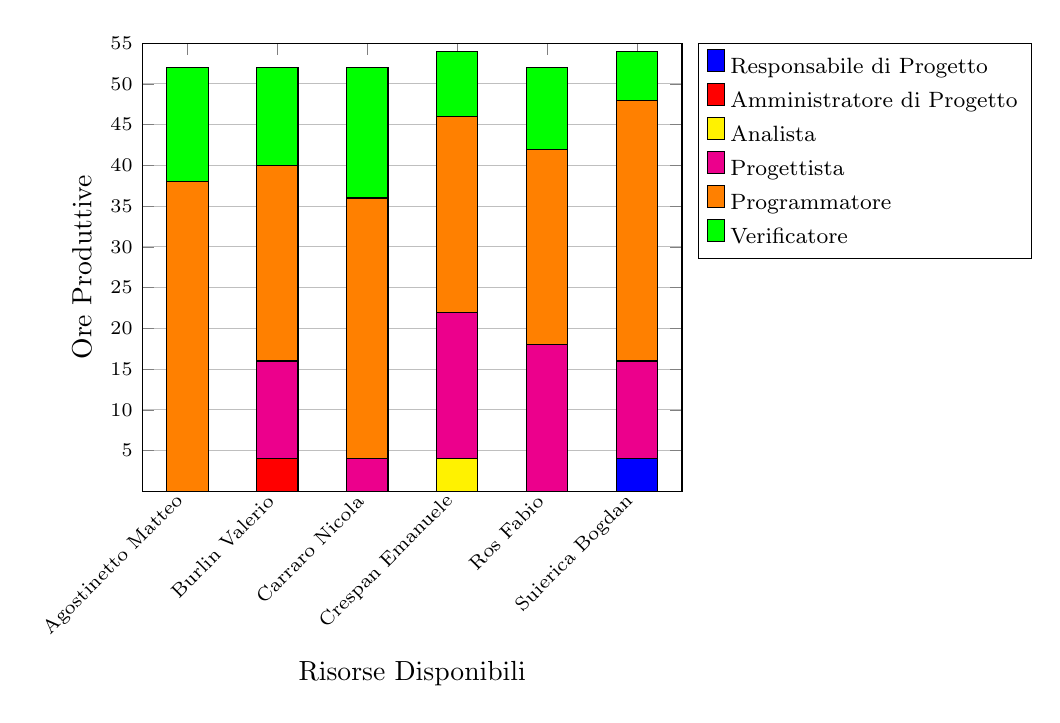
\begin{tikzpicture}
\begin{axis}[
	legend pos = outer north east,
	legend style = {nodes=right,font=\footnotesize},
	ybar stacked,
	bar width = 15pt,
	xlabel = {Risorse Disponibili},
	ylabel = {Ore Produttive},
	tick label style = {font=\scriptsize},
	symbolic x coords = {Agostinetto Matteo,Burlin Valerio,Carraro Nicola,Crespan Emanuele,Ros Fabio,Suierica Bogdan},
	xtick = data,
	x tick label style = {rotate=45,anchor=east},
	ytick = {5,10,15,20,25,30,35,40,45,50,55},
	ymajorgrids = true,
	ymin = 0,
	ymax = 55]
	\addplot+[ybar,fill = blue,draw = black]
	plot coordinates {(Agostinetto Matteo, 0) (Burlin Valerio, 0) (Carraro Nicola, 0) (Crespan Emanuele, 0) (Ros Fabio, 0) (Suierica Bogdan, 4)};
	\addplot+[ybar,fill = red,draw = black]
	plot coordinates {(Agostinetto Matteo, 0) (Burlin Valerio, 4) (Carraro Nicola, 0) (Crespan Emanuele, 0) (Ros Fabio, 0) (Suierica Bogdan, 0)};
	\addplot+[ybar,fill = yellow,draw = black]
	plot coordinates {(Agostinetto Matteo, 0) (Burlin Valerio, 0) (Carraro Nicola, 0) (Crespan Emanuele, 4) (Ros Fabio, 0) (Suierica Bogdan, 0)};
	\addplot+[ybar,fill = magenta,draw = black]
	plot coordinates {(Agostinetto Matteo, 0) (Burlin Valerio, 12) (Carraro Nicola, 4) (Crespan Emanuele, 18) (Ros Fabio, 18) (Suierica Bogdan, 12)};
	\addplot+[ybar,fill = orange,draw = black]
	plot coordinates {(Agostinetto Matteo, 38) (Burlin Valerio, 24) (Carraro Nicola, 32) (Crespan Emanuele, 24) (Ros Fabio, 24) (Suierica Bogdan, 32)};
	\addplot+[ybar,fill = green,draw = black]
	plot coordinates {(Agostinetto Matteo, 14) (Burlin Valerio, 12) (Carraro Nicola, 16) (Crespan Emanuele, 8) (Ros Fabio, 10) (Suierica Bogdan, 6)};
	\legend{\strut Responsabile di Progetto, \strut Amministratore di Progetto, \strut Analista, \strut Progettista, \strut Programmatore, \strut Verificatore}
\end{axis}
\end{tikzpicture}
\caption{Ore a componente, Progettazione di Dettaglio e Codifica}
\end{figure}
\newpage
\subsection{Verifica e Validazione}
Nella macro-fase di \textbf{Verifica e Validazione} ciascun componente del gruppo dovrà rivestire i ruoli elencati nella seguente tabella:

\begin{table}[h]
\centering
\begin{tabular}{|l|c|c|c|c|c|c|c|}
	\toprule
	\textbf{Cognome e Nome} & \multicolumn{6}{c}{\textbf{Ore per ruolo}} & \textbf{Ore Totali} \\
	& \textbf{Re} & \textbf{Am} & \textbf{An} & \textbf{Pt} & \textbf{Pr} & \textbf{Ve} & \\
		
	\midrule
	Agostinetto Matteo & & & & 10 & & 15 & 25 \\
	Burlin Valerio & & & 8 & & 8 & 9 & 25 \\ 
	Carraro Nicola & & & & 10 & & 15 & 25 \\
	Crespan Emanuele & 8 & & & & & 16 & 24 \\
	Ros Fabio & & 8 & & & 8 & 10 & 26 \\
	Suierica Bogdan & & & & 5 & & 17 & 22 \\
		
	\bottomrule
\end{tabular}
\caption{Ore a componente per ruolo, Verifica e Validazione}
\end{table}

\noindent I valori sono riassunti nel seguente grafico, che rappresenta in maniera visiva per quante ore un membro abbia ricoperto un determinato ruolo:

\begin{figure}[h]
\centering
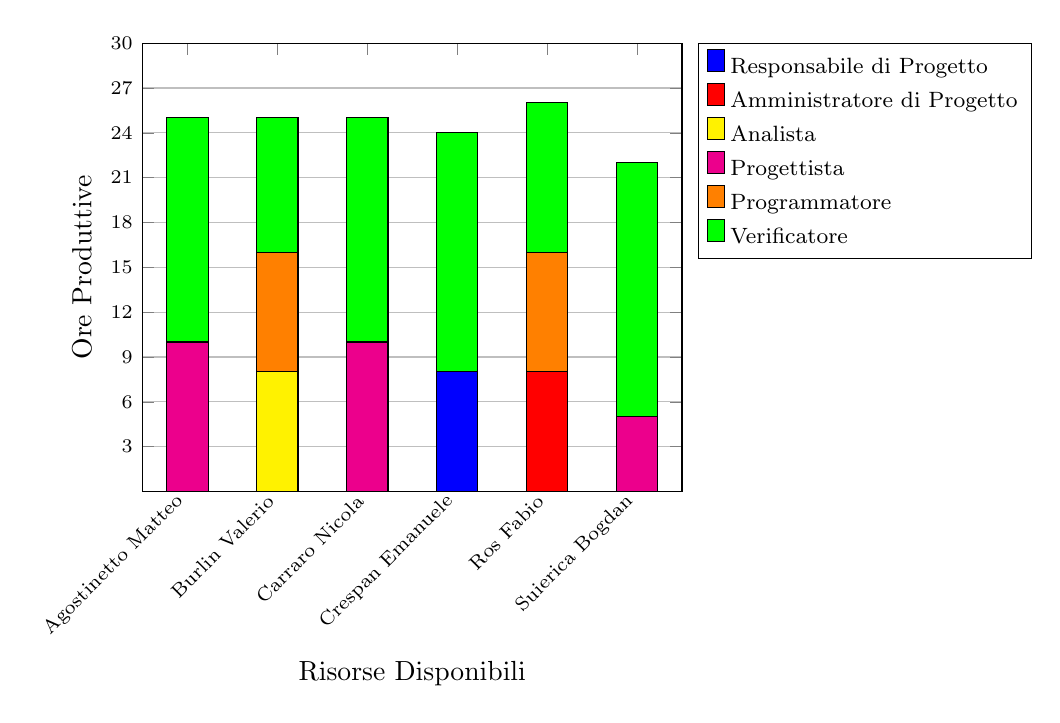
\begin{tikzpicture}
\begin{axis}[
	legend pos = outer north east,
	legend style = {nodes=right,font=\footnotesize},
	ybar stacked,
	bar width = 15pt,
	xlabel = {Risorse Disponibili},
	ylabel = {Ore Produttive},
	tick label style = {font=\scriptsize},
	symbolic x coords = {Agostinetto Matteo,Burlin Valerio,Carraro Nicola,Crespan Emanuele,Ros Fabio,Suierica Bogdan},
	xtick = data,
	x tick label style = {rotate=45,anchor=east},
	ytick = {3,6,9,12,15,18,21,24,27,30},
	ymajorgrids = true,
	ymin = 0,
	ymax = 30]
	\addplot+[ybar,fill = blue,draw = black]
	plot coordinates {(Agostinetto Matteo, 0) (Burlin Valerio, 0) (Carraro Nicola, 0) (Crespan Emanuele, 8) (Ros Fabio, 0) (Suierica Bogdan, 0)};
	\addplot+[ybar,fill = red,draw = black]
	plot coordinates {(Agostinetto Matteo, 0) (Burlin Valerio, 0) (Carraro Nicola, 0) (Crespan Emanuele, 0) (Ros Fabio, 8) (Suierica Bogdan, 0)};
	\addplot+[ybar,fill = yellow,draw = black]
	plot coordinates {(Agostinetto Matteo, 0) (Burlin Valerio, 8) (Carraro Nicola, 0) (Crespan Emanuele, 0) (Ros Fabio, 0) (Suierica Bogdan, 0)};
	\addplot+[ybar,fill = magenta,draw = black]
	plot coordinates {(Agostinetto Matteo, 10) (Burlin Valerio, 0) (Carraro Nicola, 10) (Crespan Emanuele, 0) (Ros Fabio, 0) (Suierica Bogdan, 5)};
	\addplot+[ybar,fill = orange,draw = black]
	plot coordinates {(Agostinetto Matteo, 0) (Burlin Valerio, 8) (Carraro Nicola, 0) (Crespan Emanuele, 0) (Ros Fabio, 8) (Suierica Bogdan, 0)};
	\addplot+[ybar,fill = green,draw = black]
	plot coordinates {(Agostinetto Matteo, 15) (Burlin Valerio, 9) (Carraro Nicola, 15) (Crespan Emanuele, 16) (Ros Fabio, 10) (Suierica Bogdan, 17)};
	\legend{\strut Responsabile di Progetto, \strut Amministratore di Progetto, \strut Analista, \strut Progettista, \strut Programmatore, \strut Verificatore}
\end{axis}
\end{tikzpicture}
\caption{Ore a componente, Verifica e Validazione}
\end{figure}
\newpage
\subsection{Totale}
La seguente tabella illustra le ore totali che ogni componente del gruppo dedicherà al progetto, mettendo in evidenza anche le ore che verranno poi rendicontate:

\begin{table}[h]
\centering
\begin{tabular}{|l|l|c|c|c|c|c|c|c|}
	\toprule
	\textbf{Cognome e Nome} & \multicolumn{7}{c}{\textbf{Ore per ruolo}} & \textbf{Ore Totali} \\
	& & \textbf{Re} & \textbf{Am} & \textbf{An} & \textbf{Pt} & \textbf{Pr} & \textbf{Ve} & \\
		
	\midrule
	\multirow{2}*{Agostinetto Matteo} & Totale & 3 & 5 & 16 & 26 & 38 & 45 & 133 \\
									  & Rendicontate & & 5 & & 26 & 38 & 36 & 105 \\
	\midrule
	\multirow{2}*{Burlin Valerio} & Totale & 14 & 4 & 22 & 28 & 32 & 35 & 135 \\
	                              & Rendicontate & & 4 & 16 & 28 & 32 & 25 & 105 \\ 
	\midrule
	\multirow{2}*{Carraro Nicola} & Totale & 5 & 4 & 16 & 32 & 32 & 44 & 133 \\
	                              & Rendicontate & 5 & & & 32 & 32 & 46 & 105 \\
	\midrule
	\multirow{2}*{Crespan Emanuele} & Totale & 8 & 14 & 10 & 36 & 24 & 40 & 132 \\
	                                & Rendicontate & 8 & & 4 & 36 & 24 & 33 & 105 \\
	\midrule                                
	\multirow{2}*{Ros Fabio} & Totale & 4 & 8 & 18 & 36 & 32 & 34 & 132 \\
	                         & Rendicontate & & 8 & & 36 & 32 & 29 & 105 \\ 
	\midrule                         
	\multirow{2}*{Suierica Bogdan} & Totale & 4 & 12 & 14 & 31 & 32 & 40 & 133 \\
	                               & Rendicontate & 4 & & 8 & 31 & 32 & 30 & 105 \\
	
	\bottomrule
\end{tabular}
\caption{Ore a componente per ruolo, Totali e Rendicontate}
\label{tab1}
\end{table}

\noindent Nel seguente grafico vengono visualizzate le ore totali che un membro ha ricoperto in un determinato ruolo:

\begin{figure}[h]
\centering
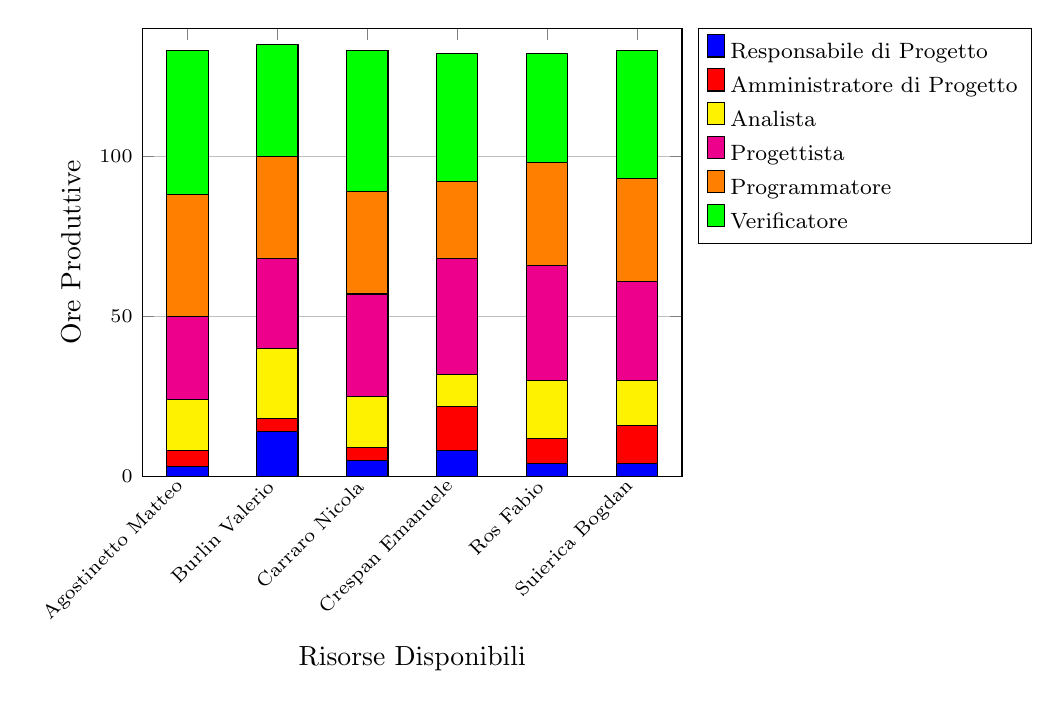
\begin{tikzpicture}
\begin{axis}[
	legend pos = outer north east,
	legend style = {nodes=right,font=\footnotesize},
	ybar stacked,
	bar width = 15pt,
	xlabel = {Risorse Disponibili},
	ylabel = {Ore Produttive},
	tick label style = {font=\scriptsize},
	symbolic x coords = {Agostinetto Matteo,Burlin Valerio,Carraro Nicola,Crespan Emanuele,Ros Fabio,Suierica Bogdan},
	xtick = data,
	x tick label style = {rotate=45,anchor=east},
	ymajorgrids = true,
	ymin = 0,
	ymax = 140]
	\addplot+[ybar,fill = blue,draw = black]
	plot coordinates {(Agostinetto Matteo, 3) (Burlin Valerio, 14) (Carraro Nicola, 5) (Crespan Emanuele, 8) (Ros Fabio, 4) (Suierica Bogdan, 4)};
	\addplot+[ybar,fill = red,draw = black]
	plot coordinates {(Agostinetto Matteo, 5) (Burlin Valerio, 4) (Carraro Nicola, 4) (Crespan Emanuele, 14) (Ros Fabio, 8) (Suierica Bogdan, 12)};
	\addplot+[ybar,fill = yellow,draw = black]
	plot coordinates {(Agostinetto Matteo, 16) (Burlin Valerio, 22) (Carraro Nicola, 16) (Crespan Emanuele, 10) (Ros Fabio, 18) (Suierica Bogdan, 14)};
	\addplot+[ybar,fill = magenta,draw = black]
	plot coordinates {(Agostinetto Matteo, 26) (Burlin Valerio, 28) (Carraro Nicola, 32) (Crespan Emanuele, 36) (Ros Fabio, 36) (Suierica Bogdan, 31)};
	\addplot+[ybar,fill = orange,draw = black]
	plot coordinates {(Agostinetto Matteo, 38) (Burlin Valerio, 32) (Carraro Nicola, 32) (Crespan Emanuele, 24) (Ros Fabio, 32) (Suierica Bogdan, 32)};
	\addplot+[ybar,fill = green,draw = black]
	plot coordinates {(Agostinetto Matteo, 45) (Burlin Valerio, 35) (Carraro Nicola, 44) (Crespan Emanuele, 40) (Ros Fabio, 34) (Suierica Bogdan, 40)};
	\legend{\strut Responsabile di Progetto, \strut Amministratore di Progetto, \strut Analista, \strut Progettista, \strut Programmatore, \strut Verificatore}
\end{axis}
\end{tikzpicture}
\caption{Ore a componente totali}
\end{figure}
\newpage

\noindent Il seguente grafico, invece, visualizza le ore rendicontate che un membro ha ricoperto in un determinato ruolo:

\begin{figure}[h]
\centering
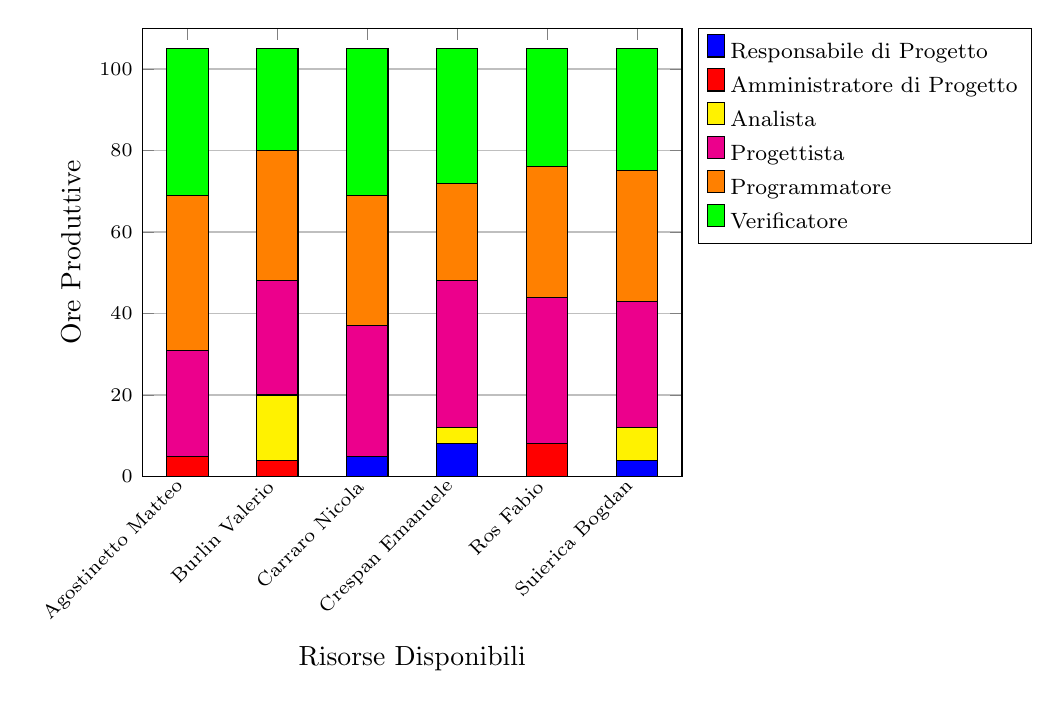
\begin{tikzpicture}
\begin{axis}[
	legend pos = outer north east,
	legend style = {nodes=right,font=\footnotesize},
	ybar stacked,
	bar width = 15pt,
	xlabel = {Risorse Disponibili},
	ylabel = {Ore Produttive},
	tick label style = {font=\scriptsize},
	symbolic x coords = {Agostinetto Matteo,Burlin Valerio,Carraro Nicola,Crespan Emanuele,Ros Fabio,Suierica Bogdan},
	xtick = data,
	x tick label style = {rotate=45,anchor=east},
	ymajorgrids = true,
	ymin = 0,
	ymax = 110]
	\addplot+[ybar,fill = blue,draw = black]
	plot coordinates {(Agostinetto Matteo, 0) (Burlin Valerio, 0) (Carraro Nicola, 5) (Crespan Emanuele, 8) (Ros Fabio, 0) (Suierica Bogdan, 4)};
	\addplot+[ybar,fill = red,draw = black]
	plot coordinates {(Agostinetto Matteo, 5) (Burlin Valerio, 4) (Carraro Nicola, 0) (Crespan Emanuele, 0) (Ros Fabio, 8) (Suierica Bogdan, 0)};
	\addplot+[ybar,fill = yellow,draw = black]
	plot coordinates {(Agostinetto Matteo, 0) (Burlin Valerio, 16) (Carraro Nicola, 0) (Crespan Emanuele, 4) (Ros Fabio, 0) (Suierica Bogdan, 8)};
	\addplot+[ybar,fill = magenta,draw = black]
	plot coordinates {(Agostinetto Matteo, 26) (Burlin Valerio, 28) (Carraro Nicola, 32) (Crespan Emanuele, 36) (Ros Fabio, 36) (Suierica Bogdan, 31)};
	\addplot+[ybar,fill = orange,draw = black]
	plot coordinates {(Agostinetto Matteo, 38) (Burlin Valerio, 32) (Carraro Nicola, 32) (Crespan Emanuele, 24) (Ros Fabio, 32) (Suierica Bogdan, 32)};
	\addplot+[ybar,fill = green,draw = black]
	plot coordinates {(Agostinetto Matteo, 36) (Burlin Valerio, 25) (Carraro Nicola, 36) (Crespan Emanuele, 33) (Ros Fabio, 29) (Suierica Bogdan, 30)};
	\legend{\strut Responsabile di Progetto, \strut Amministratore di Progetto, \strut Analista, \strut Progettista, \strut Programmatore, \strut Verificatore}
\end{axis}
\end{tikzpicture}
\caption{Ore a componente rendicontate}
\end{figure}




